% Generated from: Zhihu/专栏：概率与统计/渐近统计 (4)：弱相依数据_金鱼马_2026-06-12.md
\section{一些基本概念}

在统计分析和时间序列的领域里，我们经常遇到一些``数据之间存在依赖关系''的情况，比如每日的气温、每周的股票收益率，或者年度的GDP数值。一个基本的问题是：如何刻画并处理数据点之间依赖关系？ 这是本节主要讲解的主题。

\subsection{时间序列中的概念}

首先，平稳性假设可以提供一个稳定的统计环境，

\begin{definition*}[平稳过程]

\begin{itemize}
\tightlist
\item
  如果 $\{X(t)\}_{t\in T}$ 随时间原点的平移不改变其统计性质，即，对任意的 $n$ 和 $t_i,t_i+c\in T,\,i=1,\ldots,n$ ，随机向量 $(X(t_1),X(t_2),\dots,X(t_n))$ 和 $(X(t_1+c),X(t_2+c),\dots,X(t_n+c))$ 的分布都相同，则称 $X(t)$ 是\textbf{\emph{严平稳}} (Strict-Sense Stationary SSS) \emph{过程}。
\item
  如果 $\{X(t)\}_{t\in T}$ 满足：对任意 $t,t_1,t_2\in T$ ，其均值 $\mathbb{E}[X(t)]$ 和自相关函数 (ACF) $\mathbb{E}[X(t_1)X(t_2)]$ 不随时间原点的平移而改变，则称其为\textbf{\emph{宽平稳}} (Wide-Sense Stationary, WSS) \emph{过程}或者弱平稳过程。
\end{itemize}
\end{definition*}

此外还有诸如 $n$ 阶平稳等概念。所谓``平稳性''，都是刻画了某种角度的不变性。在本文中，我们只考虑离散时间、或者说等间隔采样的时间序列 $X_1,X_2,\dots,X_n\in\mathbb R^k$ 。

在时间序列中，一个非常经典的模型叫做\textbf{\emph{自回归滑动平均 }}(Autoregressive moving-average, ARMA) 模型，如下

\begin{definition*}[ARMA]
序列 $\{X_{t}\}_{t\in \mathbb{Z}}$ 若是宽平稳的零均值随机过程，且对任意 $t$ 满足
\[X_{t} - \theta_{1}X_{t - 1} - \dots -\theta_{p}X_{t - p} = \epsilon_{t} - \eta_{1}\epsilon_{t - 1} - \dots -\eta_{q}\epsilon_{t - q}\]
则称该序列是一个 $\mathrm{ARMA}(p,q)$ 。其中，$\{\epsilon_{t}\}$ 是一个白噪声 (white noise) 过程，记为 $\mathrm{WN}(0, \sigma^{2})$。
\end{definition*}

为了更简洁地表达，我们引入\textbf{\emph{后向移位算子 }} (backshift operator) $B$，其满足 $B^j X_t = X_{t-j}$。再定义两个多项式：

\begin{align*}
\theta(x) &= 1 - \theta_1 x - \cdots - \theta_p x^p \\
\eta(x) &= 1 - \eta_1 x - \cdots - \eta_q x^q
\end{align*}

这样，ARMA 模型就可以写成 $\theta(B)X_t = \eta(B)\epsilon_t$。它的直观理解是：当前时刻的值 $X_t$，既与过去 $p$ 个时刻的自己（AR部分）有关，也与过去 $q$ 个时刻的外部冲击（MA部分）有关。

\begin{definition*}[因果性]
设 $\{X_t\}_{t\in\mathbb Z}$ 是 $\mathrm{ARMA}(p,q)$ 过程，如果存在系数序列 $\{\psi_j\}_{j=0}^\infty$ 满足 $\sum_{j=0}^{\infty} |\psi_j| < \infty$，使得 $X_t$ 可以表示成
\[X_t = \sum_{j=0}^{\infty} \psi_j \epsilon_{t-j}\]
则称其为\textbf{\emph{因果}} (Causal) 的。
\end{definition*}

因果性保证了当前的值只依赖于过去的冲击，而不依赖于未来。这符合我们对物理世界的认知。一个因果的 $\mathrm{ARMA}(p,q)$ 过程本质上就是一个无穷阶的滑动平均过程，即 $\mathrm{MA}(\infty)$ 。

下面一个定理给出了因果性成立的充要条件：

\begin{theorem}[ARMA 过程的因果性判别]
\label{thm:ch4:arma-causality}

设 $\{X_t\}_{t\in\mathbb Z}$ 是 $\mathrm{ARMA}(p,q)$ 过程：$\theta(B)X_t=\eta(B)\epsilon_t$。若 $\theta(z)$ 和 $\eta(z)$ 没有公共零点，那么 $X_t$ 是因果的，当且仅当
\[
\theta(z)\ne 0,\qquad \forall z\in\mathbb{C},\ |z|\le 1.
\]
此时 $\psi_j$ 由 $\phi(z)=\eta(z)/\theta(z)$ 的幂级数展开确定。

(来自 \cite{brockwelldavis2006} 的 Theorem 3.1.1, pp.~85-86。)
\end{theorem}

更一般地，我们可以将 ARMA 过程置于\textbf{\emph{线性过程}} (Linear Process) 的框架下。所谓线性过程指的是：
\[X_{t} = \sum_{j = -\infty}^{\infty}\psi_{j}\epsilon_{t - j}\]
其中 $\epsilon_{t}\sim F(0,\sigma^{2})$i.i.d.。在一定条件下，ARMA 过程就是一个线性过程。

ARMA 模型虽然经典，但它假设了条件方差是恒定的。但实际中往往不满足这一点，例如，金融数据中常常出现``波动率聚集 (Volatility Clustering)''现象，即``大波动后面跟着大波动，小波动后面跟着小波动''。为了刻画这一点，Engle 提出了\textbf{\emph{自回归条件异方差}} (Autoregressive conditional heteroskedasticity, ARCH) 模型：若 $X_t$ 满足，
\[X_{t} = m(\vec{X}_{t,p}) + \sigma (\vec{X}_{t,p})\epsilon_{t}\]
则称其是一个 $\mathrm{ARCH}(p)$ ；其中 $\vec{X}_{t,p} := (X_{t - 1},\dots ,X_{t - p})^{\top}$ ， $m(\cdot)$ 和 $\sigma(\cdot)$ 分别称作条件均值函数和条件异方差函数。这个模型相较于传统的 $\mathrm{AR}(p)$ 模型 $X_t=\theta_0+\theta_1 X_{t-1}+\cdots+\theta_pX_{t-p}+\epsilon_t$，ARCH 实现了两大突破：

\begin{enumerate}
\def\labelenumi{\arabic{enumi}.}
\tightlist
\item
  将线性的条件均值函数 $m(\cdot)$ 推广到了\textbf{非线性} 形式。
\item
  将恒定的条件方差 $\sigma^2$ 推广成了一个依赖于过去信息的函数 $\sigma(\cdot)$。
\end{enumerate}

不过需要注意的是，ARCH 这类非线性模型不一定天然满足平稳性。但在一定的正则条件下，它们可以达到``渐近平稳''。读者可以参考 \cite{gourieroux2012}。

这些模型我们这里只是捎带提一下，不会深入研究。在非参数渐近理论中，我们更倾向于摆脱具体方程的束缚，转而用一种更具一般性的方式来刻画相依性，这就是混合系数。

\subsection{用混合系数度量相依性}

考虑概率空间 $(\Omega,\mathcal F,P)$ 上的随机变量序列 $\{X_t\}_{t\in\mathbb Z}$，并记 $\mathcal{F}_{l}^{m}$ 为由 $\{X_l, X_{l+1}, \dots, X_m\}$ 所生成的信息集合（子 $\sigma$-域），其中 $m>l$ 。我们可以把 $\mathcal{F}_{-\infty}^{t}$ 理解为``过去到现在''的所有信息，而 $\mathcal{F}_{t+k}^{\infty}$ 是``k 步以后直到未来''的所有信息。所谓``\textbf{\emph{弱相依}} (weak dependent)''指的是这样一种概念：当 $k \to \infty$ 时，这两部分信息的相关性应越来越小，直至近乎独立。通俗来说，序列在长远来看是``健忘''的。

以上述思路为出发点，可以定义出若干种对``相依性''的衡量，

\begin{definition*}[混合系数]
对任意两个 $\mathcal F$ 的子 $\sigma$-域 $\mathcal B,\mathcal C$，

\begin{enumerate}
\def\labelenumi{\arabic{enumi}.}
\tightlist
\item
  $\alpha$\textbf{\emph{-混合系数}}（Rosenblatt）：也称强混合 (Strong Mixing) 系数，定义为
  \[
  \alpha(\mathcal B,\mathcal C)
  :=\sup_{B\in\mathcal B,\,C\in\mathcal C}
  |P(B\cap C)-P(B)P(C)|.
  \]
  这是本文关注的重点。它的直观含义是：对于 $\mathcal{B}$ 中事件 $B$ 和 $\mathcal{C}$ 中事件 $C$，二者联合概率与它们``如果彼此独立''时应有的概率之差的最大可能值。显然 $\alpha(\mathcal{B},\mathcal{C})$ 越小，独立性越强。
\item
  \textbf{$\beta$\emph{-混合系数 }}（Kolmogorov）：也称绝对正则系数 (Absolutely Regular Coefficient)： \[ \beta(\mathcal{B},\mathcal{C}) := \mathbb{E}\left[ \sup_{C\in \mathcal{C}}\Big|P(C) - P(C|\mathcal{B})\Big| \right] \]它衡量的是：在已知所有历史信息的情况下，对未来事件 $C$ 的条件概率与无条件概率之差的期望上确界。换言之，它衡量了概率测度 $P$ 和 $P(\cdot|\mathcal B)$ 二者在 $\mathcal{C}$ 上的全变差的期望。
\item
  \textbf{$\phi$\emph{-混合系数 }}（Ibragimov; Dobrushin 等）：\[ \phi (\mathcal{B},\mathcal{C}) := \sup_{\substack{B\in \mathcal{B},C\in \mathcal{C}\\ P(B)>0}}|P(C) - P(C|B)| \]与 $\beta$-混合不同，它是在特定事件 $B$（而非整个 $\mathcal{B}$ ）条件下，概率差值的上确界。
\item
  \textbf{$\rho$\emph{-混合系数 }}（Kolmogorov \& Rozanov）：也称最大相关系数，
  \[  \rho(\mathcal{B},\mathcal{C}) := \sup_{X \in L^2(\mathcal{B}), Y \in L^2(\mathcal{C})} \Big|\operatorname{corr}(X, Y)\Big|= \sup_{X \in L^2(\mathcal{B}), Y \in L^2(\mathcal{C})}\frac{|\mathbb{E}[XY]-\mathbb{E}[X]\mathbb{E}[Y]|}{\sqrt{\mathrm{Var}[X]\mathrm{Var}[Y]}}.
  \]  其中 $L^2(\mathcal{F})$ 表示所有 $\mathcal{F}$ -可测且二阶矩有限的随机变量全体。它衡量的是过去和未来信息集中所有可能的（方差有限的）非线性变换之间的最大相关系数。
\item
  $\psi$ \textbf{\emph{-混合系数 }}（Blum, Hanson \& Koopmans）：
  \[
  \psi(\mathcal{B},\mathcal{C}):= \sup_{\substack{B\in \mathcal{B},C\in \mathcal{C}\\ P(B)>0,P(C)>0}}\left|\frac{P(B\cap C)}{P(B)P(C)}-1\right|.
  \]
\end{enumerate}

我们用 $\mathcal F_{-\infty}^t$ 和 $\mathcal F_{t+k}^\infty$ 分别代入 α-混合定义中的 $\mathcal B$ 和 $\mathcal C$ ，其结果记作 $\alpha(k)$ ，其中 $k\ge 1$ 。当 $\lim\limits_{k\to\infty}\alpha(k)=0$ 时，称序列 $X_t$ 是 $\alpha$ -混合的；其它混合系数的也可以完全类似定义。
\end{definition*}

各种混合系数之间存在着清晰的强弱关系，可以用以下不等式链和蕴含关系来总结：
\[\begin{gathered} 2\alpha(k)\le \beta(k)\le \phi(k)\le \psi(k)\\ 4\alpha(k)\le \rho(k)\le 2(\phi(k))^{1/2} \end{gathered}\]
由此可得图~\ref{fig:ch4:mixing-relations} 所示的包含关系：

\begin{figure}[htbp]
  \centering
  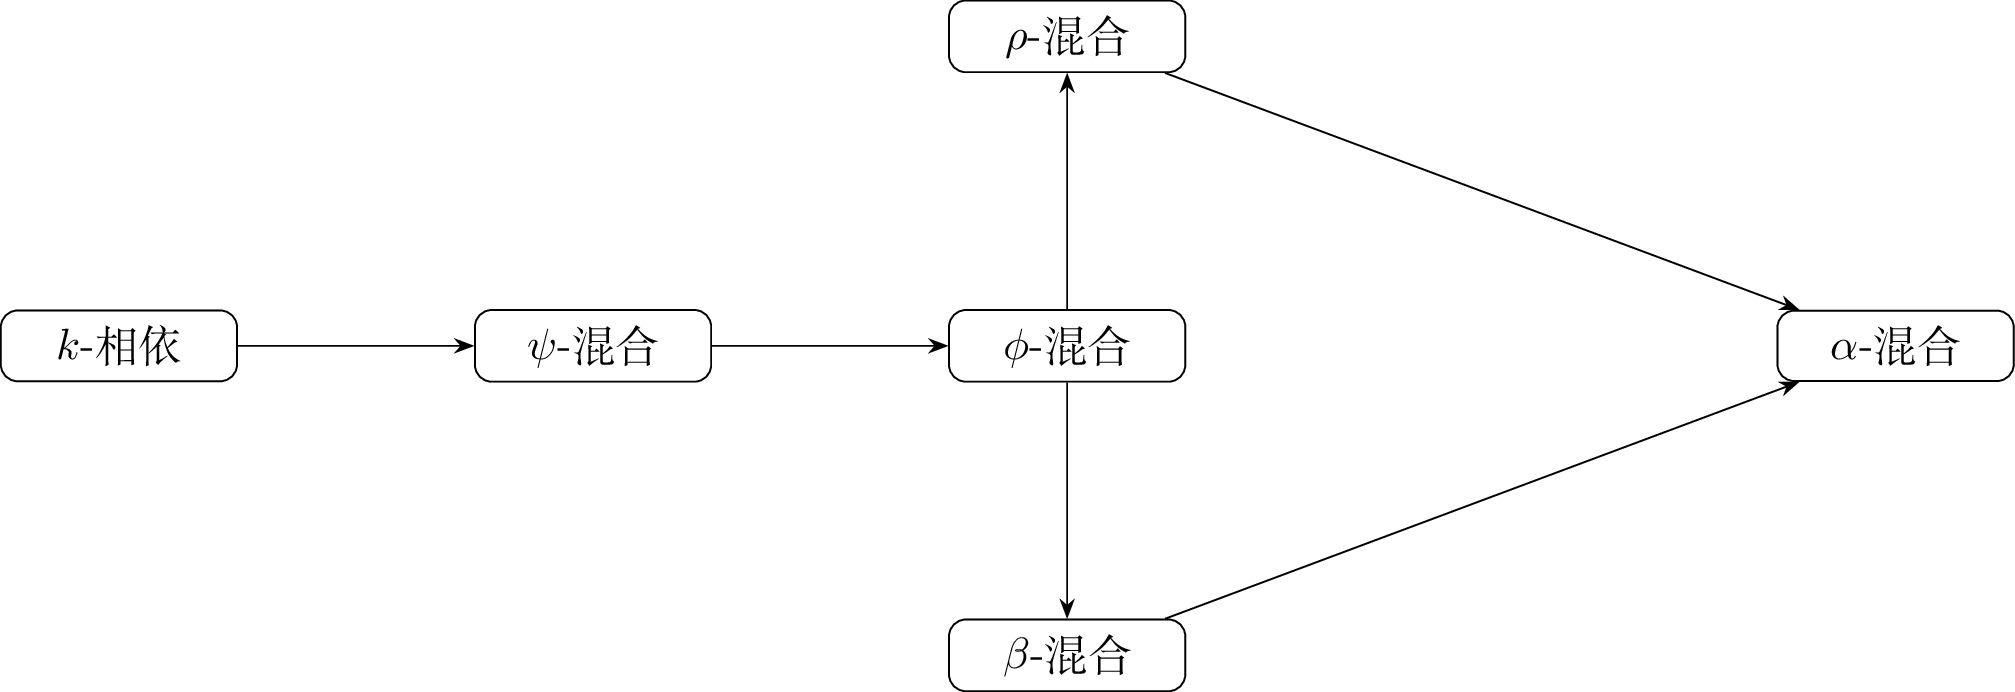
\includegraphics[width=0.94\textwidth]{figures/04-mixing-relations.png}
  \caption{各种混合条件之间的蕴含关系}
  \label{fig:ch4:mixing-relations}
\end{figure}

尽管 $\alpha$-混合的条件最弱，但它却被称作``强混合 (Strong Mixing)''，这纯属术语上的历史遗留问题。关于这些混合过程，可以参考一篇综述 \cite{bradley2005}。

一个自然的问题是：我们熟悉的模型满足这些混合性质吗？

\begin{itemize}
\tightlist
\item
  对于一个线性因果过程 $X_{t} = \sum_{j = 0}^{\infty} \psi_{j} \epsilon_{t - j}$：

\begin{itemize}
  \tightlist
  \item
    \cite{gorodetskii1978} 一文表明：在适当正则条件下， $X_t$ 是 $\alpha$ -混合的。
  \item
    如果系数 $\psi_j$ 以指数速率衰减（即 $\psi_{j} = O(\mu^{j})$，其中 $0 < \mu < 1$），那么该过程是\emph{几何 $\alpha$-混合}的，即存在常数 $C > 0$ 和 $\rho \in [0, 1)$，使得 $\alpha(k) \leq C \rho^k$。这个结论来自 \cite{tuanlanh1985}。
  \end{itemize}
\item
  对于 ARCH 过程：在一定的正则条件下，它们也具备遍历性并满足几何 $\alpha$-混合性质。例如，见 \cite{masrytjoestheim1995}。
\end{itemize}

\section{关于 α-混合系数的若干不等式}

本节证明若干 α-混合系数的基本的不等式，这些不等式表明：只要两个随机变量在时间上离得足够远，它们之间的相依性（协方差）就会被混合系数严格控制。

本节统一如下符号设定： $X,Y$ 是概率空间 $(\Omega,\mathcal F,P)$ 上的两个可积的实值随机变量， $\mathcal B,\mathcal C$ 是 $\mathcal F$ 的两个子 $\sigma$ -域，且 $X$ 为 $\mathcal B$ -可测， $Y$ 为 $\mathcal C$ -可测， $\alpha=\alpha(\mathcal B,\mathcal C)$ 。

\begin{lemma}[Billingsley 不等式]\label{lem:ch4:billingsley}

若 $|X| \leq C_1$，$|Y| \leq C_2$，那么
\[|\mathrm{Cov}(X, Y)| \leq 4C_1C_2\alpha\]
\end{lemma}

\begin{proof}

我们从协方差的定义出发，有：

\begin{equation}
\label{eq:ch4:tag-1}
|\mathrm{Cov}(X, Y)| = |\mathbb{E}[XY] -\mathbb{E}[X]\mathbb{E}[Y]| = \left|\mathbb{E}\Big[X\left(\mathbb{E}[Y|\mathcal{B}] - \mathbb{E}[Y]\right)\Big]\right|\leq C_1 \mathbb{E}\left[\Big|\mathbb{E}[Y|\mathcal{B}] - \mathbb{E}[Y]\Big|\right]
\end{equation}

令 $\xi := \operatorname{sgn}(\mathbb{E}[Y|\mathcal{B}] - \mathbb{E}[Y])$，显然 $\xi \in \mathcal{B}$ 且 $|\xi| \leq 1$。于是

\begin{equation}
\label{eq:ch4:tag-2}
\mathbb{E}\big[|\mathbb{E}[Y|\mathcal{B}] - \mathbb{E}[Y]| \big]= \mathbb{E}\left[\xi \left(\mathbb{E}[Y|\mathcal{B}] - \mathbb{E}[Y]\right)\right] = \mathbb{E}[\xi Y] - \mathbb{E}[\xi]\mathbb{E}[Y] = \mathrm{Cov}(\xi, Y)
\end{equation}

因此，

\begin{equation}
\label{eq:ch4:tag-3}
|\mathrm{Cov}(X, Y)| \leq C_1 |\mathrm{Cov}(\xi, Y)|
\end{equation}

使用同样的方法，我们对 $Y$ 和 $\xi$ 应用上述过程。令 $\eta = \operatorname{sgn}(\mathbb{E}[\xi|\mathcal{C}] - \mathbb{E}[\xi])$，则 $\eta \in \mathcal{C}$ 且 $|\eta| \leq 1$，类似地可得
\[|\mathrm{Cov}(\xi, Y)| \leq C_2 |\mathrm{Cov}(\xi, \eta)|\]
现在分析 $|\mathrm{Cov}(\xi, \eta)| = |\mathbb{E}[\xi\eta] - \mathbb{E}[\xi]\mathbb{E}[\eta]|$。由于 $\xi$ 和 $\eta$ 都是取值为 $\pm 1$ 的随机变量，我们可以通过事件概率来表示。令
\[\begin{gathered}A = \{\xi = 1\}, \quad B = \{\eta = 1\}\\ A^c = \{\xi = -1\}, \quad B^c = \{\eta = -1\} \end{gathered}\]
显然 $A, A^c \in \mathcal{B}$ 且 $B, B^c \in \mathcal{C}$。于是，
\[\begin{aligned} |\mathbb{E}[\xi\eta] - \mathbb{E}[\xi]\mathbb{E}[\eta]| &= |P(A \cap B) + P(A^c \cap B^c) - P(A^c \cap B) - P(A \cap B^c)| \\ &\leq |P(A \cap B) - P(A)P(B)| + |P(A^c \cap B^c) - P(A^c)P(B^c)| \\ &\quad + |P(A^c \cap B) - P(A^c)P(B)| + |P(A \cap B^c) - P(A)P(B^c)| \\ &\leq 4\alpha(k)  \end{aligned}\]
结合式~\eqref{eq:ch4:tag-1}、\eqref{eq:ch4:tag-2} 和 \eqref{eq:ch4:tag-3}，引理即证。

\end{proof}

\begin{lemma}[有界变量的协方差界]\label{lem:ch4:covariance-lp-bound}

若 $\mathbb{E}[|X|^{p}] < \infty$ 对某个 $p > 1$ 成立，且 $|Y| \leq C$，则
\[|\mathrm{Cov}(X, Y)| \leq 6C \|X\|_{p} \alpha^{1/q}\]
其中 $\frac{1}{p} + \frac{1}{q} = 1$，且 $\|X\|_p := (\mathbb{E}[|X|^p])^{1/p}$。

\end{lemma}

\begin{proof}

我们采用截断技术。对某个 $M > 0$，令
\[X_{M} = X\mathbb{I}(|X|\leq M), \quad X'_{M} = X - X_{M} = X\mathbb{I}(|X| > M)\]
则 $X = X_{M} + X'_{M}$。根据协方差的线性性质，
\[|\mathrm{Cov}(X,Y)| = |\mathrm{Cov}(X_{M},Y) + \mathrm{Cov}(X_{M}^{\prime},Y)|\leq |\mathrm{Cov}(X_{M},Y)| + |\mathrm{Cov}(X'_{M},Y)|\]
首先处理第一项。由于 $|X_M| \leq M$ 且 $|Y| \leq C$，由引理~\ref{lem:ch4:billingsley} 有

\begin{equation}
\label{eq:ch4:tag-4}
|\mathrm{Cov}(X_{M},Y)|\leq 4CM\alpha
\end{equation}

其次处理第二项，我们有
\[\begin{aligned} \mathbb{E}[|X_{M}'|] &= \int_{|X| > M}|x|\mathrm{d}F(x) \\ &\leq \int_{|X| > M}|x|\left(\frac{|x|}{M}\right)^{p-1}\mathrm{d}F(x) \\ &\leq M^{-(p-1)}\int_{-\infty}^{\infty} |x|^p \mathrm{d}F(x) = M^{1-p}\mathbb{E}[|X|^{p}] \end{aligned}\]
因此，

\begin{equation}
\label{eq:ch4:tag-5}
|\mathrm{Cov}(X_M',Y)| = |\mathbb{E}[X_M'Y] - \mathbb{E}[X_M']\mathbb{E}[Y]| \leq \mathbb{E}[|X_M'Y|] + C\mathbb{E}[|X_M'|] \leq 2C\mathbb{E}[|X_M'|] \leq 2C M^{1-p}\mathbb{E}[|X|^p]
\end{equation}

现在，为了最小化式~\eqref{eq:ch4:tag-4} 和 \eqref{eq:ch4:tag-5} 的和，我们选择 $M$ 使得两项平衡。取
\[M = \| X\| _p\alpha ^{- 1 / p}\]
将 $M$ 分别代入式~\eqref{eq:ch4:tag-4} 和 \eqref{eq:ch4:tag-5}：
\[|\mathrm{Cov}(X_{M},Y)|\leq 4C \| X\| _p\alpha ^{- 1 / p} \alpha  = 4C \| X\| _p \alpha^{1 - 1/p} = 4C \| X\| _p\alpha^{1/q}\]\[|\mathrm{Cov}(X_M',Y)| \leq 2C \left(\| X\| _p \alpha^{-1/p}\right)^{1-p} \mathbb{E}[|X|^p] = 2C \| X\| _p^{1-p} \alpha^{(p-1)/p} \| X\| _p^p = 2C \| X\| _p \alpha^{1/q}\]
将两式相加即证。

\end{proof}

引理~\ref{lem:ch4:covariance-lp-bound} 是引理~\ref{lem:ch4:billingsley} 的推广：后者只是前者在 $p=\infty,q=1$ 的特例。

\begin{lemma}[Rio 不等式]\label{lem:ch4:rio}

令 $Q_{X}(u) = \inf \{t: P(|X| > t) \leq u\}$ 为 $|X|$ 的分位数函数。如果 $Q_{X}Q_{Y}$ 在 $(0,1)$ 上可积，则
\[|\mathrm {Cov}(X,Y)|\leq 2\int_{0}^{2\alpha}Q_{X}(u)Q_{Y}(u)\mathrm{d}u\]
\end{lemma}

\begin{proof}

我们将随机变量 $X$ 和 $Y$ 分解为其正部和负部：$X = X^{+} - X^{-}$，$Y = Y^{+} - Y^{-}$，其中 $X^{+} = \max(0, X)$，$X^{-} = \max(0, -X)$。利用协方差的线性性质，可得

\begin{equation}
\label{eq:ch4:tag-6}
\mathrm{Cov}(X,Y) = \mathrm{Cov}(X^{+},Y^{+}) + \mathrm{Cov}(X^{-},Y^{-}) - \mathrm{Cov}(X^{-},Y^{+}) - \mathrm{Cov}(X^{+},Y^{-})
\end{equation}

对于任意两个非负随机变量 $U$ 和 $V$，不难验证其协方差可以写作：

\begin{equation}
\label{eq:ch4:tag-7}
\mathrm{Cov}(U,V) = \int_{0}^{\infty} \!\!\int_{0}^{\infty} \Big( P(U > u, V > v) - P(U > u)P(V > v) \Big)\mathrm{d}u \mathrm{d}v
\end{equation}

将此式应用于 $X^{+}$ 和 $Y^{+}$，我们得到：
\[\mathrm{Cov}(X^{+},Y^{+}) = \int_{0}^{\infty} \!\!\int_{0}^{\infty} \Big( P(X^{+} > u, Y^{+} > v) - P(X^{+} > u)P(Y^{+} > v) \Big)  \mathrm{d}u  \mathrm{d}v\]
根据 $\alpha$-混合系数的定义，对任意事件 $A \in \sigma(X)$ 和 $B \in \sigma(Y)$，有 $|P(A \cap B) - P(A)P(B)| \leq \alpha$。同时，联合概率 $P(A \cap B)$ 显然不会超过边缘概率 $P(A)$ 或 $P(B)$。因此，被积函数中的概率差值的绝对值可以被 $\min \big\{\alpha, P(X^{+} > u), P(Y^{+} > v) \big\}$ 所控制。从而有：
\[\mathrm{Cov}(X^{+},Y^{+}) \leq \int_{0}^{\infty} \!\!\int_{0}^{\infty}\min \big\{ \alpha, P(X^{+} > u), P(Y^{+} > v) \big\} \mathrm{d}u  \mathrm{d}v\]
我们将式~\eqref{eq:ch4:tag-6} 中的四项协方差全部用形如式~\eqref{eq:ch4:tag-7} 的形式进行放缩，并利用如下的初等结论：对任意非负实数 $a, b, c, d$ 和 $\alpha > 0$，有
\[(\alpha \wedge a \wedge c) + (\alpha \wedge a \wedge d) + (\alpha \wedge b \wedge c) + (\alpha \wedge b \wedge d) \leq 2\big[ (2\alpha) \wedge (a + b) \wedge (c + d) \big]\]
将此不等式应用于 $a = P(X > u), b = P(-X > u), c = P(Y > v), d = P(-Y > v)$ ，我们可以将四项积分合并，得到：
\[|\mathrm{Cov}(X,Y)| \leq 2\int_{0}^{\infty} \!\!\int_{0}^{\infty}\min \big\{ 2\alpha, P(|X| > u), P(|Y| > v) \big\} \mathrm{d}u  \mathrm{d}v =: \mathcal{I}\]
最后一步是证明积分 $\mathcal{I}$ 等于定理中给出的形式。考虑均匀分布随机变量 $U\sim\mathcal U([0,1])$，并基于它定义：
\[Z:=\begin{cases} Q_X(U),&\text{ 若 }U<2\alpha\\ 0,&\text{ 若 }U\ge 2\alpha \end{cases}\quad T:=\begin{cases} Q_Y(U),&\text{ 若 }U<2\alpha\\ 0,&\text{ 若 }U\ge 2\alpha \end{cases}\]
则有：
\[\mathbb{E}[ZT] = \int_{0}^{2\alpha} Q_{X}(u) Q_{Y}(u) \, \mathrm{d}u\]
另一方面，事件 $\{Z > u, T > v\}$ 发生当且仅当 $U < 2\alpha$ 且同时满足 $U < P(|X| > u)$ 和 $U < P(|Y| > v)$。因此，
\[P(Z > u, T > v) = \mathbb{P}\big(U < 2\alpha, U < P(|X| > u), U < P(|Y| > v) \big) = \min\big\{ 2\alpha, P(|X| > u), P(|Y| > v) \}\]
由于 $Z$ 和 $T$ 非负，我们再次使用前述积分恒等式，得到：
\[\mathbb{E}[ZT] =\int_{0}^{\infty} \!\!\int_{0}^{\infty}P(Z > u, T > v) \mathrm{d}u \mathrm{d}v = \int_{0}^{\infty} \!\!\int_{0}^{\infty}\min\big\{ 2\alpha, P(|X| > u), P(|Y| > v) \big\}  \mathrm{d}u \mathrm{d}v = \frac{1}{2} \mathcal{I}\]
比较 $\mathbb{E}[ZT]$ 的两个表达式，便有 $\mathcal{I} = 2 \int_{0}^{2\alpha} Q_{X}(u) Q_{Y}(u) \, \mathrm{d}u$。

\end{proof}

利用引理~\ref{lem:ch4:rio}，我们可推导出经典的 Davydov 不等式，这是处理混合相依序列矩不等式的一项核心工具，

\begin{lemma}[Davydov 不等式]\label{lem:ch4:davydov}

令 $X$ 和 $Y$ 满足 $X \in L^q(\mathcal{B})$，$Y \in L^r(\mathcal{C})$，其中 $q > 1$，$r > 1$ 且 $\frac{1}{q} + \frac{1}{r} = 1 - \frac{1}{p}$，则
\[|\mathrm{Cov}(X, Y)| \leq 2p(2\alpha(k))^{1/p} \|X\|_q \|Y\|_r\]
\end{lemma}

\begin{proof}

分三种情况。

\begin{enumerate}
\def\labelenumi{\arabic{enumi}.}
\tightlist
\item
  $q$ 和 $r$ 均为有限的情形
\end{enumerate}

由 Markov 不等式，
\[P\left(|X| > \frac{\|X\|_q}{u^{1 / q}}\right) \leq \frac{\mathbb{E}|X|^q}{\left(\|X\|_q / u^{1 / q}\right)^q} = u, \quad 0 < u \leq 1\]
根据分位数函数 $Q_X$ 的定义，上式说明
\[Q_X(u) \leq \frac{\|X\|_q}{u^{1 / q}}, \quad 0 < u \leq 1\]
类似地，$Q_Y(u) \leq \|Y\|_r / u^{1 / r}$。使用 Rio 不等式（引理~\ref{lem:ch4:rio}），
\[\begin{aligned} |\mathrm {Cov}(X, Y)| & \leq 2 \int_0^{2\alpha} \frac{\|X\|_q \|Y\|_r}{u^{1 / q} u^{1 / r}} \mathrm{d}u \\ & = 2 \|X\|_q \|Y\|_r \int_0^{2\alpha} u^{\frac{1}{p} - 1} \mathrm{d}u \\ & = 2 p(2\alpha )^{1 / p} \|X\|_q \|Y\|_r \end{aligned}\]
\begin{enumerate}
\def\labelenumi{\arabic{enumi}.}
\setcounter{enumi}{1}
\tightlist
\item
  $r = \infty$，$q$ 有限的情形
\end{enumerate}

此时 $\frac{1}{q} + \frac{1}{p} = 1$。注意到， $Q_Y(u) \leq Q_Y(0) = \|Y\|_\infty = \sup |Y|$ ，再次用 Rio 不等式，
\[| \mathrm{Cov}(X, Y) | \leq 2 \int_0^{2\alpha} \frac{\|X\|_q}{u^{1/q}} \|Y\|_\infty \mathrm{d}u = 2 \|X\|_q \|Y\|_\infty \int_0^{2\alpha} u^{\frac{1}{p}-1} \mathrm{d}u = 2p(2\alpha)^{1/p} \|X\|_q \|Y\|_\infty\]
这与引理~\ref{lem:ch4:covariance-lp-bound} 相似但不全相同。

\begin{enumerate}
\def\labelenumi{\arabic{enumi}.}
\setcounter{enumi}{2}
\tightlist
\item
  $r = +\infty$ 且 $q = +\infty$ 的情形
\end{enumerate}

此时 $p = 1$。再次使用 Rio 不等式，
\[|\mathrm {Cov}(X,Y)|\leq 2\int_{0}^{2\alpha }\| X\|_{\infty}\| Y\|_{\infty}\mathrm{d}u = 4\| X\|_{\infty}\| Y\|_{\infty}\alpha\]
这与引理~\ref{lem:ch4:billingsley} 完全相同。

\end{proof}

关于这些不等式，推荐读者参考 \cite{bosq1996} 一书的第一章。也可参阅 \cite{lulingzhengyan1997} 一书的 §1.2。

最后给出 Davydov 不等式（引理~\ref{lem:ch4:davydov}）的一个具体应用。

\begin{definition*}[长记忆与短记忆过程]
设 $\{X_t\}_{t\in\mathbb Z}$ 是一个二阶矩有限的宽平稳过程。令 $\gamma(k)=\mathrm{Cov}(X_i,X_{i+k})$ 是其自协方差函数 (ACVF)。

\begin{itemize}
\tightlist
\item
  如果 $\sum_{k=0}^{\infty} |\gamma(k)| = \infty$，则它是一个\textbf{\emph{长记忆过程}} (Long Memory Process)。
\item
  如果 $\sum_{k=0}^{\infty} |\gamma(k)| < \infty$，我们称该过程为\textbf{\emph{短记忆过程}} (Short Memory Process) 。
\end{itemize}
\end{definition*}

长记忆与短记忆这两个术语最早见 \cite{mcleodhipel1978}。

利用 Davydov 不等式（取 $r = q$），如果 $\mathbb{E}[|X_i|^q ]< \infty$ 对 $q > 2$ 成立，且 $\sum_{k = 0}^{\infty} (\alpha(k))^{1 / p} < \infty$ 对 $p = \frac{q}{q - 2}$ 成立，则
\[\sum_{k=0}^\infty|\gamma(k)|\le 2p\|X\|_q^2\sum_{k=0}^\infty(\alpha(k))^{1/p}<\infty\]
说明该过程是短记忆的。

特别地，如果 $\alpha (k) \leq C \rho^k$ ，即``几何强混合 (GSM)''，则
\[\sum_{k = 0}^{\infty} (\alpha(k))^{1 / p} \leq C \sum_{k = 0}^{\infty} \rho^{k / p} = \frac{C}{1 - \rho^{1 / p}} < \infty .\]
通常，为了保证 $\sum_{k=0}^\infty (\alpha(k))^{1/p} < \infty$，只需要 $(\alpha(k))^{1/p} \sim k^{-(1+\eta)}$，即当 $k$ 充分大时 $\alpha(k) \sim k^{-p(1+\eta)}$ 对某个 $\eta > 0$ 成立；几何强混合意味着 $\alpha(k) \leq C\rho^k$，其衰减速度是指数级的，条件更强。

\section{α-混合序列的中心极限定理}

关于混合相依变量的弱收敛，有非常多的理论，除了本节要介绍的 α-混合序列中心极限定理外，还有一些研究放宽了矩条件或平稳性条件，或是研究其它混合系数下的弱收敛，或是弱不变原理等；除了这些渐近结论，还有类比于 Hoeffding 不等式、Bernstein 不等式这样的非渐近不等式（但对于相依序列而言结论十分复杂，并且其界与混合系数有关）。限于篇幅，无法一一叙述。

\subsection{准备工作}

首先的一个结论可以类比于弱大数律：

\begin{theorem}[长程方差的存在性]
\label{thm:ch4:long-run-variance}

令 $\{X_t\}_{t \in \mathbb{Z}}$ 是一个零均值、实值的弱平稳过程，满足对某个 $r > 2$，
\[\sup_{t\in \mathbb{Z}}\mathbb{E}[|X_t|^r ]< \infty ,\quad \sum_{k\geq 1}\alpha (k)^{1 - \frac{2}{r}}< \infty\]
则级数 $\sum_{k\in \mathbb{Z}}\gamma (k)$ 绝对收敛，且收敛到一个非负和 $\sigma^2$，使得
\[\lim_{n\to \infty}n\mathrm{Var}(S_n / n) = \sigma^2\]
其中 $\gamma (k) := \mathrm{Cov}(X_i, X_{i+k})$ 是自协方差函数， $S_n:=\sum_{t=1}^nX_t$ 代表连续 $n$ 项和。

\end{theorem}

\begin{remark}

\begin{itemize}
\tightlist
\item
  注意，由于宽平稳性， $\gamma(k)=\mathrm{Cov}(X_i,X_{i+k})$ 的值和 $i$ 无关；同样， $S_n$ 的起点选择也和其分布无关。
\item
  这里的 $\sigma^2$ 又叫做\textbf{\emph{长程方差}} (Long-run Variance)。
\end{itemize}
\end{remark}

\begin{proof}

首先我们研究级数 $\sum_{k \in \mathbb{Z}} \gamma(k)$ 的收敛性。使用 Davydov 不等式（引理~\ref{lem:ch4:davydov}），取 $q = r$ 且 $\frac{1}{p} = 1 - \frac{2}{r}$，得到
\[|\gamma (k)| \leq 2p (2\alpha(k))^{1/p} \|X_0\|_r \|X_k\|_r \leq 2p (2\alpha(k))^{1 - 2/r} \sup_{t\in\mathbb{Z}}\|X_t\|_r^2\]
由于 $\sum_{k \geq 1} \alpha (k)^{1 - 2 / r} < +\infty$，根据比较判别法，级数 $\sum_k |\gamma(k)|$ 绝对收敛。

现在考虑 $n \mathrm{Var} (S_n / n)$，
\[n \mathrm{Var}\! \left(\frac{S_n}{n}\right) = n^{-1} \sum_{0 \leq s, t \leq n - 1} \mathrm{Cov}(X_s, X_t) = \sum_{k = -(n - 1)}^{n - 1} \left(1 - \frac{|k|}{n}\right) \gamma (k)\]
根据控制收敛定理，当 $n \to \infty$ 时，
\[\lim_{n \to \infty} n \mathrm{Var}\! \left(\frac{S_n}{n}\right) = \sum_{k=-\infty}^\infty \gamma(k) = \sigma^2 \geq 0\]
定理得证。

\end{proof}

第二个工具叫做\textbf{\emph{耦合方法}} (Coupling Method) ，这是一种将``变量间存在依赖性的平稳随机序列''转变为``彼此独立的随机变量序列''的手段。简而言之，给定一个具有复杂相依关系的随机向量 $(X,Y)\in\mathbb R^k\times\mathbb R$，我们构造一个新的随机变量 $Y^*$，使得它与 $Y$ 同分布，但与 $X$ 独立，并且 $Y^*$ 和 $Y$ 尽可能接近。相关的结论如下：

\begin{lemma}[Bradley 引理]\label{lem:ch4:bradley}

令随机向量 $(X,Y)\in \mathbb{R}^d\times \mathbb{R}$ ，满足 $Y\in L^p(P)$ ， $p\in [1,\infty)$。令 $c$ 为一个实数，使得 $\| Y + c\| _p > 0$，并令 $\xi \in (0,\| Y + c\| _p]$。则存在一个随机变量 $Y^{*}$ 满足：

\begin{enumerate}
\def\labelenumi{\arabic{enumi}.}
\tightlist
\item
  $P_{Y^{*}} = P_{Y}$ ；
\item
  $Y^{*}$ 与 $X$ 独立；
\item
  \[
  P(|Y-Y^*|>\xi)
  \leq 11(\xi^{-1}\|Y+c\|_p)^{p/(2p+1)}
  \bigl(\alpha(\sigma(X),\sigma(Y))\bigr)^{2p/(2p+1)}.
  \]
\end{enumerate}

\end{lemma}
来自 \cite{bradley1983} 一文的 Theorem 3。在该论文中，这里的常数 11 原本是 18 且 $c = 0$，但证明过程是一致的。

最后还有一个引理，帮助我们后文中阶的估算


\begin{lemma}[横山良三矩界]\label{lem:ch4:yokoyama}

设 $\{X_t\}_{t\in \mathbb Z}$ 是零均值、实值、严平稳的 α-混合过程，满足：存在 $\gamma>2$ 和 $\delta>0$ 使得 $\mathbb{E}[|X_t|^{\gamma+\delta}] < \infty$ 。若
\[
\sum_{k=1}^\infty(k+1)^{\gamma/2-1}(\alpha(k))^{\frac\delta{\gamma+\delta}}<\infty,
\]

那么存在常数 $C$ 使得对每个 $n\ge 1$ ， $\mathbb{E}[|S_n|^\gamma]\le Cn^{\gamma/2}$

\end{lemma}
该引理来自 \cite{yokoyama1980} 一文的 Theorem 1。


\begin{corollary}\label{cor:ch4:moment-bound}
设 $\{X_t\}_{t\in \mathbb Z}$ 是零均值实值严平稳过程，满足：存在 $\gamma > 2$ 和 $\beta > 1$，使得
\[\mathbb{E}[|X_t|^\gamma] < \infty , \quad \alpha (k) \leq a k^{-\beta}\]
其中 $a$ 为正常数，且 $\beta > \gamma / (\gamma - 2)$。那么存在常数 $C$ 和 $\gamma'\in(2,\gamma)$ 使得对每个 $n\ge 1$，$\mathbb{E}[|S_n|^{\gamma'}]\le Cn^{\gamma'/2}$。
\end{corollary}

\begin{proof}

根据引理~\ref{lem:ch4:yokoyama}，我们只需证明 
$$\sum_{k=1}^\infty(k+1)^{\gamma'/2-1}(\alpha(k))^{\frac{\gamma-\gamma'}{\gamma}}<\infty$$
代入 $\alpha (k) \leq a k^{-\beta}$ ，上式等价于 $\frac{\gamma'}2-1-\beta\frac{\gamma-\gamma'}{\gamma}<-1$ ，即 $\gamma'<\frac{2\beta\gamma}{2\beta+\gamma}$ 。另一方面， $\beta > \gamma / (\gamma - 2)$ 保证了 $\frac{2\beta\gamma}{2\beta+\gamma}=((2\beta)^{-1}+\gamma^{-1})^{-1}>((2\gamma/(\gamma-2))^{-1}+\gamma^{-1})^{-1}=2$ ，即区间 $\left(2,\frac{2\beta\gamma}{2\beta+\gamma}\right)$ 非空，总是可以做到从中取 $\gamma'$ 的。

\end{proof}

\subsection{α-混合序列的中心极限定理和证明}

对严平稳 α-混合随机序列，I. A. Ibragimov 最早给出了其中心极限定理的充要条件，但相当繁琐，不易验证。下面的定理是一个充分条件， 来自 \cite{bosq1996} 书中的 Theorem 1.7。

\begin{theorem}[$\alpha$-混合序列的中心极限定理]
\label{thm:ch4:alpha-mixing-clt}

令 $\{X_{t}\}_{t\in \mathbb{Z}}$ 是零均值实值严平稳过程，满足：存在 $\gamma > 2$ 和 $\beta > 1$， 使得
\[\mathbb{E}[|X_t|^\gamma] < \infty , \quad \alpha (k) \leq a k^{-\beta}\]
其中 $a$ 为正常数，且 $\beta > \gamma / (\gamma - 2)$。如果 $\sigma^2 = \sum_{k = -\infty}^{\infty} \gamma (k) > 0$，则有
\[\frac{S_n}{\sigma\sqrt{n}} \overset{\rm d}\to\mathcal N(0,1)\]
\end{theorem}

\begin{proof}

为清晰起见，我们分成六步。

\emph{第一步}：首先，由定理~\ref{thm:ch4:long-run-variance}，我们知道自协方差 $\gamma(k)$ 满足绝对收敛 $\sum_{k=-\infty}^\infty |\gamma(k)| < \infty$，从而 $\sigma^2$ 是良定义的。

\emph{第二步}：应用 \textbf{\emph{Bernstein Blocking Method }}：将序列 $X_1,\dots,X_n$ 分割为长度为 $p$ 的大块和长度为 $q$ 的小块，按``大块-小块-大块-小块-\ldots{}''交替排列，并让其长度满足：

\begin{itemize}
\tightlist
\item
  $p\sim\frac n{\log n}-n^{1/4}$ ；
\item
  $q\sim n^{1/4}$ 。
\end{itemize}

则共有 $r:=\left[\frac n{p+q}\right]\sim \log n$ 个大块和小块，并且由于被小块分隔开的缘故，大块之间是近似独立的。

记大块内随机变量的和为 $Y_i$ ，小块内的和为 $Z_i$ ， $i=1,\dots,r$ ，从而 $S_n$ 可写作
\[
\begin{aligned}
S_n={}&\underbrace{(X_1+ \cdots+ X_p)}_{Y_1} + \underbrace{(X_{p+1}+ \dots +X_{p+q})}_{Z_1}\\
&+ \underbrace{(X_{p+q+1} +\dots +X_{2p+q})}_{Y_2}+ \underbrace{(X_{2p+q+1}+ \dots +X_{2p+2q})}_{Z_2}+\dots\\
&+ \underbrace{(X_{(r-1)(p+q)+1} +\dots +X_{rp+(r-1)q})}_{Y_r}\\
&+\underbrace{(X_{rp+(r-1)q+1}+ \dots +X_{r(p+q)})}_{Z_r} + \text{余项 } R_r.
\end{aligned}
\]
第三步：考虑对每个大块应用 Bradley 引理（引理~\ref{lem:ch4:bradley}），从而得到一系列独立的副本 $Y^*_i$ ，且 $Y_i$ 与 $Y^*_i$ 足够接近。我们按照如下方式构造副本 $Y_i^*$：

\begin{itemize}
\tightlist
\item
  对于 $i = 1$ ，取 $Y_1^*=Y_1$ ；
\item
  对于 $i \ge 2$，将 Bradley 引理应用于：$(Y_1,Y_2,\dots,Y_{i-1})$ 和 $Y_i$，得到 $Y_i^*$ 。取常数 $c = \zeta p \|X_0\|_\gamma$（ $\zeta > 1$ ）、 $\xi = \frac{\epsilon \sigma \sqrt{n}}{r}$（ $\epsilon > 0$ 充分小）。此时对足够大的 $n$，
  \[
  \|Y_i+c\|_\gamma
  \ge c-\|Y_i\|_\gamma
  \ge (\zeta-1)p\|X_0\|_\gamma
  \ge \frac{\epsilon\sigma\sqrt n}{r}
  =\xi,
  \]
  从而 Bradley 引理的条件成立；上面最后一个不等式用到了 $p\sim\frac n{\log n}$ 的阶大于 $\frac{\sqrt n}r\sim\frac{\sqrt n}{\log n}$ 的阶。
\end{itemize}

由此得到了 i.i.d. 的 $Y_1^*,\dots,Y_r^*$ ，且\[ P\left( |Y_i - Y^*_i| > \frac{\epsilon \sigma \sqrt{n}}{r} \right) \leq 11 \left( \frac{\|Y_i + c\|_\gamma}{\xi} \right)^{\frac{\gamma}{2\gamma+1}} \alpha(q)^{\frac{2\gamma}{2\gamma+1}} \] 对 $i$ 求和，记\[ \Delta_n := \frac{\sum_{i=1}^r Y_i}{\sigma \sqrt{n}} - \frac{\sum_{i=1}^r Y^*_i}{\sigma \sqrt{n}} = \frac{1}{\sigma\sqrt{n}} \sum_{i=1}^r (Y_i - Y^*_i) \]

则
\[P(|\Delta_n| > \epsilon) \leq \sum_{i=1}^r P\left( |Y_i - Y^*_i| > \frac{\epsilon \sigma \sqrt{n}}{r} \right) \leq 11 r \left( \frac{\|Y_1 + c\|_\gamma}{\xi} \right)^{\frac{\gamma}{2\gamma+1}} \alpha(q)^{\frac{2\gamma}{2\gamma+1}}.\]记上式右侧为 $m_n$，由 $\|Y_i+c\|_\gamma/\xi=O(pr/\sqrt n)=O(\sqrt n)$，可知 $m_n$ 的阶数为
\[\begin{aligned}m_n &= O\left( r \cdot n^{\frac{\gamma}{4\gamma+2}} \cdot \alpha([n^{1/4}])^{\frac{2\gamma}{2\gamma+1}} \right)\\ &= O\left( \log n\cdot n^{\frac{\gamma}{4\gamma+2}} \cdot n^{-\frac{\beta \gamma}{2(2\gamma+1)}} \right)\\ &=O\left(\log n\cdot n^{-\frac{(\beta-1)\gamma}{4\gamma+2}}\right)\\ &\to 0 \end{aligned}\]
即 $\Delta_n\overset{P}\to 0$ 。

第五步：我们表明上一步中构造的 i.i.d. 副本 $Y_1^*,\dots,Y_n^*$ 满足中心极限定理。首先，显然 \[ \mathbb{E}\big[{Y^*_i}^2\big]=\mathbb{E}[Y_i^2]=\mathbb{E}[S_p^2]\sim \sigma^2p \]由推论~\ref{cor:ch4:moment-bound}，存在 $2<\gamma'<\gamma$ 使得 $\mathbb{E}[|Y_i|^{\gamma'}]\le Cp^{\gamma'/2}$，$i=1,\dots,r$。从而
\[
\begin{aligned}
\sum_{i=1}^r
\frac{\mathbb E[|Y^*_j|^{\gamma'}]}
{\left(\mathrm{Var}\left[\sum_{i=1}^rY^*_j\right]\right)^{\gamma'/2}}
&=O\left(r\frac{Cp^{\gamma'/2}}{(r\sigma^2p)^{\gamma'/2}}\right)\\
&=O\left(r^{1-\gamma'/2}\right)\to 0.
\end{aligned}
\]
Lyapunov 条件得以满足，独立和 $\sum_{j=1}^r Y_j^*$ 的中心极限定理成立：
\[\frac{Y_1^*+\cdots+Y_n^*}{\sigma\sqrt n}=\underbrace{\left(\frac{rp}{n}\right)^{1/2}}_{\to 1}\frac{Y_1^*+\cdots+Y_n^*}{\sigma\sqrt{rp}}\overset{\rm d}\to \mathcal N(0,1)\]
从而，根据 Slutsky 定理， \[ \frac{Y_1+\cdots+Y_n}{\sigma\sqrt n}=\frac{Y_1^*+\cdots+Y_n^*}{\sigma\sqrt n}+\underbrace{\Delta_n}_{o_P(1)}\overset{\rm d}\to\mathcal N(0,1) \]第六步：与四、五步完全相同地，对小块也有中心极限定理成立： \[ \frac{Z_1+\cdots+Z_n}{\sigma\sqrt{rq}}\overset{\rm d}\to \mathcal N(0,1) \]那么 \[ \frac{Z_1+\cdots+Z_n}{\sigma\sqrt{n}}=\underbrace{\left(\frac{rq}{n}\right)^{1/2}}_{\to 0}\frac{Z_1+\cdots+Z_n}{\sigma\sqrt{rq}}\to 0 \]所以根据 Slutsky 定理，小块的部分是可忽略的。

至于尾部余项 $R_r$，由于其长度不超过 $p+q$，由 Chebyshev 不等式，
\[P\left( \frac{|R_r|}{\sigma \sqrt{n}} > \epsilon \right) \leq \frac{\mathrm{Var}(R_r)}{\epsilon^2 \sigma^2 n} = O\left( \frac{\sigma^2(p+q)}{\epsilon^2\sigma^2n} \right) = O\left( \frac{1}{\log n} \right) \to 0\]
自然也是可忽略的。至此，我们完成了证明。

\end{proof}

最后，我们整理一下上述证明思路：

\begin{itemize}
\tightlist
\item
  定理~\ref{thm:ch4:long-run-variance} 保证 $\sigma^2$ 存在且有限。
\item
  用 Bernstein Blocking Method 将 $X_1,X_2,\dots,X_n$ 划分为大块、以及把大块分隔开的小块。
\item
  用 Bradley 引理为每个大块内元素和 $Y_i$ 提供独立同分布的副本 $Y_i^*$ 。
\item
  证明副本 $Y_i^*$ 满足 Lyapunov 中心极限定理。
\item
  副本 $Y_i^*$ 和原来的 $Y_i$ 之间的差距是可忽略的，小块和余项也是可忽略的，所以总体便成立中心极限定理。
\end{itemize}

\section{如何估计长程方差？------谱方法入门}

根据定理~\ref{thm:ch4:alpha-mixing-clt}， $S_n/\sqrt n$ 的渐近方差就是所谓的长程方差 $\sigma^2 = \sum_{k=-\infty}^\infty \gamma(k)=\gamma(0)+2\sum_{k=1}^\infty\gamma(k)$。如果我们能有对 $\sigma^2$ 的很好的估计，就能解决构建置信区间、或是进行假设检验等统计问题。但如何从数据中估计这个包含了所有自协方差的量呢？通常的方法是借助频域谱分析。

\subsection{谱密度函数}

\begin{definition*}[谱分布函数与谱密度函数]
对于实值宽平稳过程 $\{X(t)\}_{t\in T}$ 和其自协方差函数 $\gamma(k)$，如果有 $[-\pi,\pi]$ 上单调不减右连续的函数 $F(\lambda)$ 使得 $F(-\pi)=0$，且对每个 $k\in\mathbb Z$ 成立 $\gamma(k)=\int_{-\pi}^\pi e^{ik\lambda}\mathrm{d}F(\lambda)$，则称 $F(\lambda)$ 是 $X(t)$ 或 $\gamma(k)$ 的\textbf{\emph{谱分布函数}} (spectral distribution function)。如果有 $[-\pi,\pi]$ 上的非负函数 $f(\lambda)$ 使得对每个 $k\in\mathbb Z$ 成立 $\gamma(k)=\int_{-\pi}^\pi f(\lambda)e^{ik\lambda}\mathrm{d}\lambda$，则称 $f(\lambda)$ 是 $X(t)$ 或 $\gamma(k)$ 的\textbf{\emph{谱密度函数}} (spectral density function)，又称功率谱。
\end{definition*}

Herglotz 定理保证了 $F(\lambda)$ 的唯一存在性。若 $F(\lambda)$ 和 $f(\lambda)$ 同时存在，则 $F(\lambda)=\int_{-\pi}^\lambda f(s)\mathrm{d}s$ 。

关于谱密度函数，更常见的另一种定义如下，当 $\gamma(k)$ 绝对可和（即级数绝对收敛）： $\sum_{-\infty}^\infty |\gamma(k)|<\infty$ ，则 \[ f(\lambda)=\frac1{2\pi}\sum_{k=-\infty}^\infty e^{ik\lambda}\gamma(k) \]就是谱密度函数。可见 \cite{brockwelldavis2006} 一书的 Theorem 4.3.2 和 Corollary 4.3.2 等。进一步，由 Weierstrass M-判别法，上述级数一致收敛，从而 $f(\lambda)$ 在 $[-\pi,\pi]$ 上一致连续。

\begin{example}[ARMA 过程的谱密度]
设有 $\mathrm{ARMA}(p,q)$ 过程 $\theta(B)X_t = \eta(B)\epsilon_t$，$\epsilon_t\sim \mathrm{WN}(0, \sigma^2)$，满足定理~\ref{thm:ch4:arma-causality} 的因果性条件，使得 $X_t=\psi(B)\epsilon_t=\sum_{j=0}^\infty\psi_j\epsilon_{t-j}$，其中 $\psi(z)=\frac{\eta(z)}{\theta(z)}=\sum\limits_{j=0}^\infty\psi_jz^j,\enspace |z|\le 1$。其自协方差函数为（不失一般性设 $k\ge 0$）：
\[\begin{aligned} \gamma(k)&=\mathbb{E}[X_tX_{t+k}]\\ &=\mathbb{E}\!\left[\left(\sum_{j=0}^\infty\psi_j\epsilon_{t-j}\right)\left(\sum_{l=0}^\infty\psi_l\epsilon_{t+k-l}\right)\right]\\ &=\sum_{j=0}^\infty\sum_{l=0}^\infty \psi_j\psi_l\mathbb{E}[\epsilon_{t+j}\epsilon_{t+k-l}]\\ &=\sigma^2\sum_{j=0}^\infty\psi_j\psi_{j+k} \end{aligned}\]
其中最后一行来自于白噪声有\[ \mathbb{E}[\epsilon_{t-j} \epsilon_{t+k-l}] = \begin{cases} \sigma^2, & \text{若 } j = l-k, \\ 0, & \text{ 其它 } \end{cases} \]
从而，谱密度函数就是
\[\begin{aligned} f(\omega) &= \frac{\sigma^2}{2\pi} \sum_{k=-\infty}^{\infty} \sum_{j=0}^{\infty} \psi_j \psi_{j+|k|} e^{-i k \omega} \\ &= \frac{\sigma^2}{2\pi} \sum_{j=0}^{\infty} \sum_{m=0}^{\infty} \psi_j \psi_m e^{-i (j-m) \omega}   \\ &= \frac{\sigma^2}{2\pi} \left( \sum_{j=0}^{\infty} \psi_j e^{-i j \omega} \right) \left( \sum_{m=0}^{\infty} \psi_m e^{i m \omega} \right) \\ &= \frac{\sigma^2}{2\pi} \left| \sum_{j=0}^{\infty} \psi_j e^{-i j \omega} \right|^2 \end{aligned}\]
注意到 $\sum_{j=0}^{\infty} \psi_j e^{-i j \omega} = \psi(e^{-i\omega})$，因此 $\mathrm{ARMA}(p,q)$ 的谱密度函数最终可写作：
\[f(\omega)=\frac{\sigma^2}{2\pi}\left|\frac{\eta(e^{-i\omega})}{\theta(e^{-i\omega})}\right|^2\]

\end{example}

显而易见， \[ \sigma^2=\sum_{k=-\infty}^\infty \gamma(k)=2\pi f(0) \]即：信号在零频率处的能量，恰好等于时域信号所有时间点上相关性的总和。估计长程方差 $\sigma^2$ 等价于估计谱密度在零频率处的值 $f(0)$ ；我们的问题化作：如何估计谱密度函数？

\subsection{周期图}

\textbf{\emph{周期图}} (Periodogram) 是 $f(\lambda)$ 直接在样本上的对应：

\begin{definition}[周期图]
  $\{X_1, \dots , X_n\}$ 的周期图在 Fourier 频率 $\omega_j = 2\pi j / n \in [-\pi , \pi]$ 处定义为
\[I_n(\omega_j) = \frac1n\left|\sum_{t = 1}^{n}X_t e^{-it\omega_j}\right|^2,\quad j\in T = \{0,\pm 1,\ldots ,\pm [n / 2]\}\]\end{definition}

图~\ref{fig:ch4:periodogram} 是一个例子，其中 $n=100$ ；原始的时间序列信号数值在 -3 到 +3 之间波动，表现为高频率的震荡，而周期图把时间域的信号转换到频率域，在大约 17 附近有一个尖峰，说明信号在这个频率附近有很强的成分。

\begin{figure}%[htbp]
  \centering
  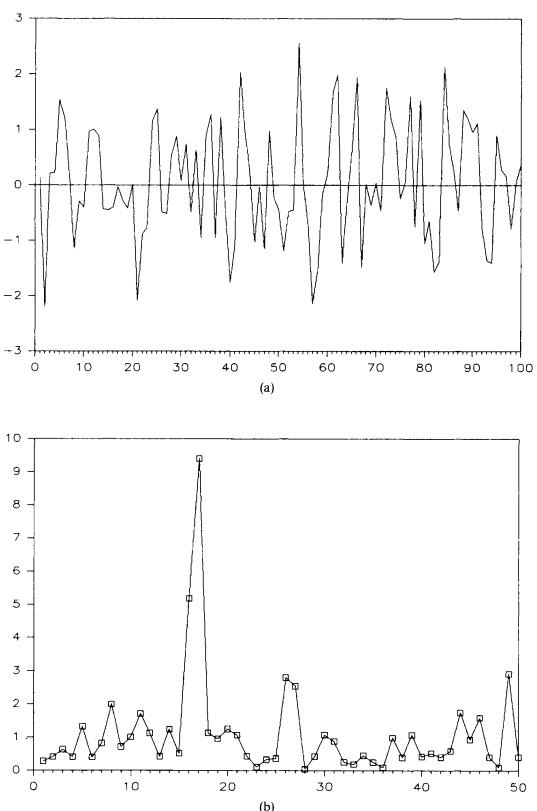
\includegraphics[height=0.5\textheight]{figures/04-periodogram-example.png}
  \caption{时间序列及其周期图。图片来自 \cite{brockwelldavis2006}, p.~340}
  \label{fig:ch4:periodogram}
\end{figure}

记
\[\begin{aligned} \bar{X}&:=\frac1n\sum_{t=1}^nX_i\\ \widehat\gamma(k)&:=\frac1n\sum_{t=1}^{n-|k|}(X_t-\bar{X})(X_{t+k}-\bar{X}) \end{aligned}\]
那么可以看出 $I_n(0)=n|\bar X|^2$ ；且当 $\omega_j\ne 0$ 时，

\begin{equation}
\label{eq:ch4:tag-8}
\begin{aligned} I_n(\omega_j)& = \frac1n\left|\sum_{t = 1}^{n}X_t e^{-it\omega_j}\right|^2\\ &=\frac1n\left|\sum_{t = 1}^{n}(X_t-\bar{X}) e^{-it\omega_j}\right|^2\\ &=\frac1n\sum_{t=1}^n\sum_{s=1}^n(X_t-\bar{X})(X_s-\bar{X})e^{-i(t-s)\omega_j}\\ &=\sum_{k=-(n-1)}^{n-1}e^{-ik\omega_j}\left(\frac1n\sum_{t=1}^{n-|k|}(X_t-\bar{X})(X_{t+|k|}-\bar{X})\right)\\ &=\sum_{|k|<n}\widehat\gamma(k)e^{-ik\omega_j} \end{aligned}
\end{equation}

接下来，我们把周期图延拓到 $[-\pi,\pi]$ 上：对任意 $\omega\in[-\pi,\pi]$ ，定义周期图为\[ I_n(\omega):=\begin{cases} I_n(\omega_k),&\text{ 若 }\omega_k-\frac\pi n<\omega\le \omega_k+\frac\pi n\text{ 且 }0\le\omega\le \pi\\ I_n(-\omega)&\text{ 若 }-\pi\le\omega<0 \end{cases} \]
即：在 $[0,\pi]$ 上，让 $I_n(\omega)$ 取值为最接近 $\omega$ 的那个 $\omega_k=\frac{2\pi j}{n}$ 的周期图；在 $[-\pi,0)$ 上直接对称过来；据此，可以构造一个映射 $g_n(\omega):[-\pi,\pi]\to \{2\pi j/n\}_{j=0,\pm1,\dots,\pm[n/2]}$ ，使得 $I_n(g_n(\omega))=I_n(\omega)$ 。

我们证明下述周期图的渐近性质：

\begin{theorem}[周期图的渐近无偏性]\label{thm:ch4:periodogram-expectation}

设 $\{X_t\}_{t\in\mathbb Z}$ 平稳，有均值为 $\mu$，且自协方差函数 $\gamma(\cdot)$ 绝对可和，则
\[\mathbb{E}[I_n(0)] - n\mu^2 \to 2\pi f(0) \quad \text{且} \quad \mathbb{E}[I_n(\omega)] \to 2\pi f(\omega) \quad \text{如果 } \omega \neq 0\]
如果 $\mu = 0$，则 $\mathbb{E}[I_n(\omega)]$ 在 $[-\pi, \pi]$ 上一致收敛到 $2\pi f(\omega)$。

\end{theorem}

\begin{proof}

首先，由定理~\ref{thm:ch4:long-run-variance}，
\[\mathbb{E}[I_n(0)] - n\mu^2 = n\mathbb{E}[|\bar{X}|^2] - n\mu^2 = n \mathrm{Var}(\bar{X}) = n \mathrm{Var}(S_n/n) \to \sum_{k=-\infty}^\infty \gamma(k) = 2\pi f(0)\]
现在如果 $\omega \in (0, \pi]$，则对充分大的 $n$，有 $g_n( \omega) \neq 0$。因此，由式~\eqref{eq:ch4:tag-8}，
\[\begin{aligned} \mathbb{E}[I_n(\omega)] &=\mathbb{E}[I_n(g_n(\omega))] \\ &=\sum_{|k|< n} \left(\frac1n\sum_{t = 1}^{n - |k|}\mathbb{E}[(X_{t} - \mu)(X_{t + |k|} - \mu)]\right)e^{-i k g_n(\omega)} \\ &= \sum_{|k|< n}\left(1 - \frac{|k|}{n}\right)\gamma (k)e^{-i k g_n(\omega)}  \end{aligned}\]
由于 $\gamma(\cdot)$ 绝对可和，级数 $\sum_{|k|< n}\left(1 - \frac{|k|}{n}\right)\gamma (k)e^{- i k\lambda}$ 在 $\lambda$ 上一致收敛到 $2\pi f(\lambda)$。因此，由于 $g_n(\omega) \to \omega$ 当 $n \to \infty$，我们有
\[\mathbb{E}[I_n(\omega)]\to 2\pi f(\omega)\]
当 $\mu = 0$ 时，利用 $f$ 在 $[-\pi,\pi]$ 上的一致连续性以及 $g_n(\omega)$ 在 $[0,\pi]$ 上一致收敛到 $\omega$ 可验证一致收敛性。

\end{proof}

定理~\ref{thm:ch4:periodogram-expectation} 的结论可以阐述为：若 $\omega\ne 0$，那么将 $\frac{I_n(\omega)}{2\pi}$ 作为 $f(\omega)$ 的估计量是渐近无偏的。

如果是线性过程，还有更精细的收敛结论，如下，

\begin{theorem}[周期图的有限维极限]
\label{thm:ch4:periodogram-limit}

令 $\{X_{t}\}_{t\in\mathbb Z}$ 为线性过程，满足 $X_{t} = \sum_{j = -\infty}^{\infty} \psi_j \epsilon_{t - j}$，其中 $\epsilon_{t}\sim F(0, \sigma^{2})$ i.i.d.，且 $\sum_{j = -\infty}^{\infty} |\psi_{j}| < \infty$。令 $I_{n}(\lambda)$ 表示 $\{X_{1}, \dots , X_{n}\}$ 的周期图， $f (\lambda)$ 为 $\{X_{t}\}_{t\in\mathbb Z}$ 的谱密度。

\begin{enumerate}
\def\labelenumi{\arabic{enumi}.}
\tightlist
\item
  如果对所有的 $\lambda \in [-\pi, \pi]$ 均有 $f(\lambda) > 0$，且 $0 < \lambda_{1} < \dots < \lambda_{m} < \pi$，则当 $n\to\infty$ 时随机向量 $(I_{n}(\lambda_{1}), \dots , I_{n}(\lambda_{m}))^{\top}$ 依分布收敛于一个随机向量，该向量的各个分量相互独立，且第 $i$ 个分量服从均值为 $2\pi f(\lambda_{i})$ 的指数分布。
\item
  如果进一步假设系数满足更强的衰减条件 $\sum_{j = -\infty}^{\infty} |\psi_{j}| |j|^{1/2} < \infty$，且 $\mathbb{E}[\epsilon_{1}^{4}] = \eta \sigma^{4} < \infty$，并令 $\omega_s = 2\pi s / n \geq 0$ 和 $\omega_t = 2\pi t / n \geq 0$ 为 Fourier 频率，则周期图在不同频率处的协方差具有如下精确的渐近展开：
  \[  \mathrm{Cov}(I_n(\omega_s), I_n(\omega_t)) = \begin{cases} 2(2\pi)^2 f^2(\omega_s) + O(n^{-1/2}) & \text{若 } \omega_s = \omega_t = 0 \text{ 或 } \pi, \\ (2\pi)^2 f^2(\omega_s) + O(n^{-1/2}) & \text{若 } 0 < \omega_s = \omega_t < \pi, \\ O(n^{-1}) & \text{若 } \omega_s \neq \omega_t. \end{cases}
  \]  其中，$O(n^{-1/2})$ 项与 $O(n^{-1})$ 项关于 $s$ 和 $t$ 是一致有界的。
\end{enumerate}

\end{theorem}

\begin{remark}

\begin{itemize}
\tightlist
\item
  定理~\ref{thm:ch4:periodogram-limit} 的证明见 \cite{brockwelldavis2006} 一书的 Theorem 10.3.2。除此之外，前文涉及的周期图相关结论和定理~\ref{thm:ch4:periodogram-expectation} 也见本书 Proposition 10.1.2、Proposition 10.3.1。
\item
  关于谱密度的估计，另一可参考的资料是 \cite{brillinger2001} 一书第 5 章。
\end{itemize}
\end{remark}

由定理~\ref{thm:ch4:periodogram-limit} 可见，如果我们用周期图 $\frac{I_n(\omega)}{2\pi}$ 来估计谱密度函数 $f(\omega)$，其方差不会随着样本量增加而消失，所以周期图 $\frac{I_n(\omega)}{2\pi}$ \emph{不是}谱密度的相合估计。这是我们不愿看到的：对参数 $\theta$，一个好的估计量 $\hat{\theta}_n$ 至少应当是相合的，即当 $n \to \infty$ 时，$\hat{\theta}_n$ 应依概率收敛到 $\theta$。

其原因在于：在经典的统计学中，样本量 $n$ 的增加通常意味着我们在同一个参数上获得了更多的独立观测，因此估计量的方差会以 $O(1/n)$ 下降；但在频域里，样本量 $n$ 的增加只是意味着我们在 $[-\pi, \pi]$ 上能分辨出更更多的点，而并没有在某一个特定的频率上增加重复观测。

然而有失有得：从定理~\ref{thm:ch4:periodogram-limit} 中还可以看到，当 $n$ 较大时且 $\omega_s\ne \omega_t$ 时，$\mathrm{Cov}(I_n(\omega_s), I_n(\omega_t))=O(n^{-1})\to 0$，说明周期图在各频率点上的纵坐标近似不相关；同时，由功率谱函数 $f(\lambda)$ 的连续性，在一个足够小的区间内，$I_n(\omega)$ 的方差也变化不大，因此我们有望通过在 $\lambda$ 的一个小邻域内对周期图纵坐标进行平均，来构造 $f(\lambda)$ 的相合估计量。本质上，这与经典统计中``通过样本平均消除随机误差以构造相合估计''是相同的。

\subsection{离散谱平均估计}

大多数传统方法采用的是一种称之为``周期图平滑''------或者叫``加窗''的方法，即用下述``\textbf{\emph{离散谱平均估计}} (discrete spectral average estimator)''：
\[
\widehat{f}(\omega_j)=\frac1{2\pi}\sum_{|k|\le m_n}W_n(k)I_n(\omega_{j+k}),
\]
作为谱密度的估计，其中 $W_n(\cdot)$ 满足

\begin{itemize}
\tightlist
\item
  当 $n\to\infty$ 时， $m_n\to\infty$ 但 $m_n/n\to 0$ ；
\item
  对每个 $k$ ， $W_n(k)=W_n(-k)$ ；
\item
  $\sum_{|k|\le m_n}W_n(k)=1$ ；
\item
  当 $n\to\infty$ 时， $\sum_{|k|\le m_n}W_n^2(k)\to 0$ 。
\end{itemize}

简而言之，我们用 $W_n(k)$ 作为权重，将 $-m_n\le k\le m_n$ 这段区域中的 $I_n(\omega_{j+k})$ 进行加权平均，以得到 $f(\omega_j)$ 的估计；这一过程如图~\ref{fig:ch4:spectral-smoothing} 所示。

\begin{figure}[htbp]
  \centering
  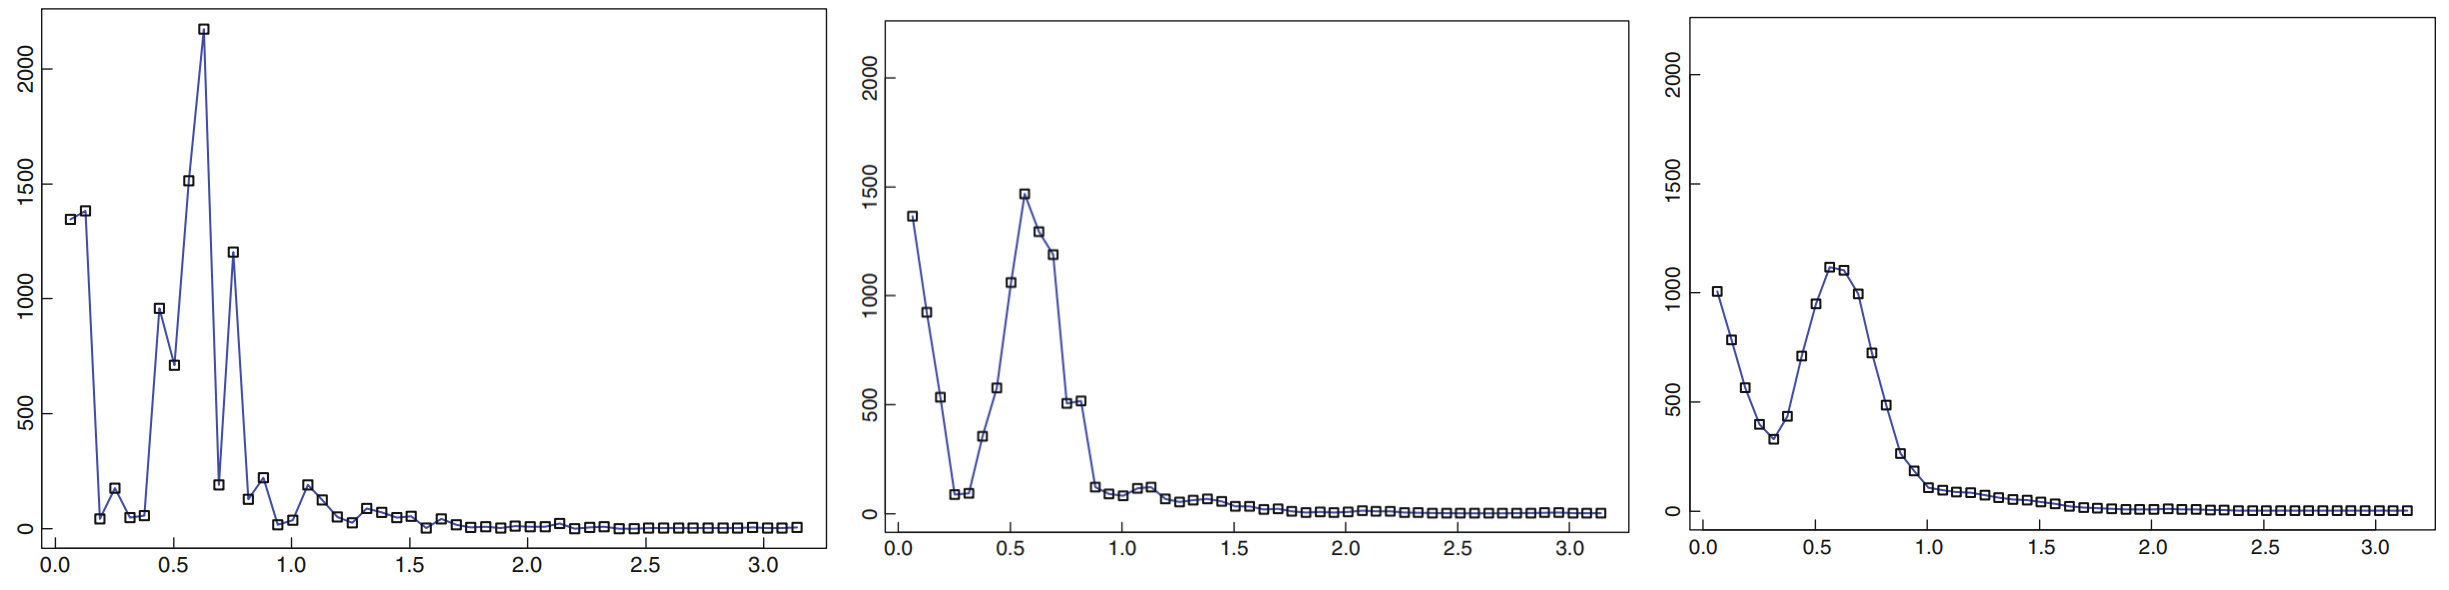
\includegraphics[width=0.96\textwidth]{figures/04-spectral-smoothing.png}
  \caption{离散谱平均估计的示意图。图片来自 \cite{brockwelldavis2006}, \S4.2}
  \label{fig:ch4:spectral-smoothing}
\end{figure}

类似于谱密度函数，用 $\widehat{f}(\omega)=\widehat f(g_n(\omega))$ 将 $\widehat f$ 延拓到 $[-\pi,\pi]$ 上。我们可以看到定理~\ref{thm:ch4:periodogram-limit} 的结果可以得到改进：

\begin{theorem}[离散谱平均估计的相合性]\label{thm:ch4:spectral-average-consistency}

令 $\{X_{t}\}_{t\in\mathbb Z}$ 为线性过程，满足 $X_{t} = \sum_{j = -\infty}^{\infty} \psi_j \epsilon_{t - j}$，其中 $\epsilon_{t}\sim F(0, \sigma^{2})$ i.i.d.，且 $\sum_{j = -\infty}^{\infty} |\psi_{j}| |j|^{1/2} < \infty$ ， $\mathbb{E}[\epsilon_1^4]<\infty$ 。那么谱平均估计 $\widehat f$ 满足：

\begin{itemize}
\tightlist
\item
  （渐近无偏）对 $\lambda\in[0,\pi]$ ， $\lim\limits_{n\to\infty}\mathbb{E}\big[\widehat f(\lambda)\big]=f(\lambda)$ ；
\item
  （相合性）对 $\omega_t,\omega_s\in[0,\pi]$，
  \[  \lim_{n \to \infty} \left( \sum_{|j| \leq m_n} W_n^2(j) \right)^{-1} \mathrm{Cov}\big[\widehat{f}(\omega_t), \widehat{f}(\omega_s)\big] = \begin{cases} 2f^2(\omega) & \text{ 若 } \omega_t = \omega_s = 0 \text{ 或 } \pi, \\ f^2(\omega) & \text{ 若 } 0 < \omega_t = \omega_s < \pi, \\ 0 & \text{ 若 } \omega_t \neq \omega_s. \end{cases}
  \]  这蕴含了 $\mathrm{Var}\big[\widehat f(\omega)\big]\sim f^2(\omega)\sum\limits_{|k|\le m_n}W_n^2(j)\to 0$ 。
\end{itemize}

\end{theorem}


见 \cite{brockwelldavis2006} 一书的 Theorem 10.4.1。

\subsection{非参数回归}

另一种思路称作``对数周期图回归''。注意到定理~\ref{thm:ch4:periodogram-limit} 导出了一个回归模型：
\[I_n(\omega_{j}) = (2\pi)f (\omega_{j})e_{j} + R_j,\quad j\in T\]
其中 $e_j\sim\mathrm{Exp}(1)$ i.i.d.，而 $R_j$ 是可忽略的项。（注意，根据定理~\ref{thm:ch4:periodogram-expectation}， $I_{n}(0)$ 可能是有偏的，如有必要我们从 $T$ 中剔除掉 $\{0\}$ ）。

将上式两边取对数，并忽略掉 $R_j$ ，
\[\log\left(\frac{I_{n}(\omega_j)}{2\pi}\right) = \log f (\omega_j) + \log e_j,\quad j\in T\]
这里 $\log e_j$ 服从 Gumbel 分布，有 $\mathbb{E}[\log(e_j)] = -0.57721\ldots$（Euler 常数），$\mathrm{Var}(\log(e_j)) = \pi^2 /6$。 令 $\eta_j := \log(e_j) + 0.57721\dots$，$W_j := \log(I_n(\omega_j) / (2\pi)) + 0.57721\ldots$，$m(\omega) := \log f(\omega)$，便得到如下固定设计 (fixed-design) 非参数回归模型：
\[W_{j} = m(\omega_{j}) + \eta_{j}, \quad j \in T\]
其中 $\{\eta_{j}\}$ i.i.d.，均值为零，方差 $\sigma_{\eta}^{2} = \pi^{2} / 6$。

我们可以通过``滑动平均''来估计 $m(0) = \log f(0)$。基于核函数 $K$ 和平滑带宽 (smoothing bandwidth) $b$ 的 $m(\omega)$ 的 \textbf{\emph{Nadaraya-Watson估计量 }} 为
\[\widehat{m}_b(\omega) = \frac{\sum_{j\in T } K\left(\frac{\omega - \omega_j}{b}\right) W_j}{\sum_{j\in T } K\left(\frac{\omega - \omega_j}{b}\right)}\]
其中当 $n\to\infty$ 时 $b \to 0$ 且 $nb \to \infty$ 。 最终，$f(0)$ 的估计量为 $\widehat{f}(0) = \exp(\widehat{m}_b(0))$。
